\documentclass[12pt, border=8pt]{standalone}
\usepackage{tikz}
\usepackage{amsmath, amssymb, bm}
\usepackage{xcolor}
\usetikzlibrary{positioning, arrows.meta, calc, fit, backgrounds}

% ── Colour aliases ──────────────────────────────────────────────────────────
\definecolor{forgetred}{RGB}{192,57,43}       % c0392b
\definecolor{inputgreen}{RGB}{39,174,96}      % 27ae60
\definecolor{candidateblue}{RGB}{41,128,185}  % 2980b9
\definecolor{outputorange}{RGB}{211,84,0}     % d35400
\definecolor{highwayorange}{RGB}{230,126,34}  % e67e22
\definecolor{arrowblue}{RGB}{79,134,198}      % 4f86c6
\definecolor{tanhbg}{RGB}{254,249,231}        % fef9e7
\definecolor{tanhborder}{RGB}{243,156,18}     % f39c12

\begin{document}
\pagestyle{empty}

  \textbf{LSTM Cell --- Gate Architecture}

\vspace{4pt}

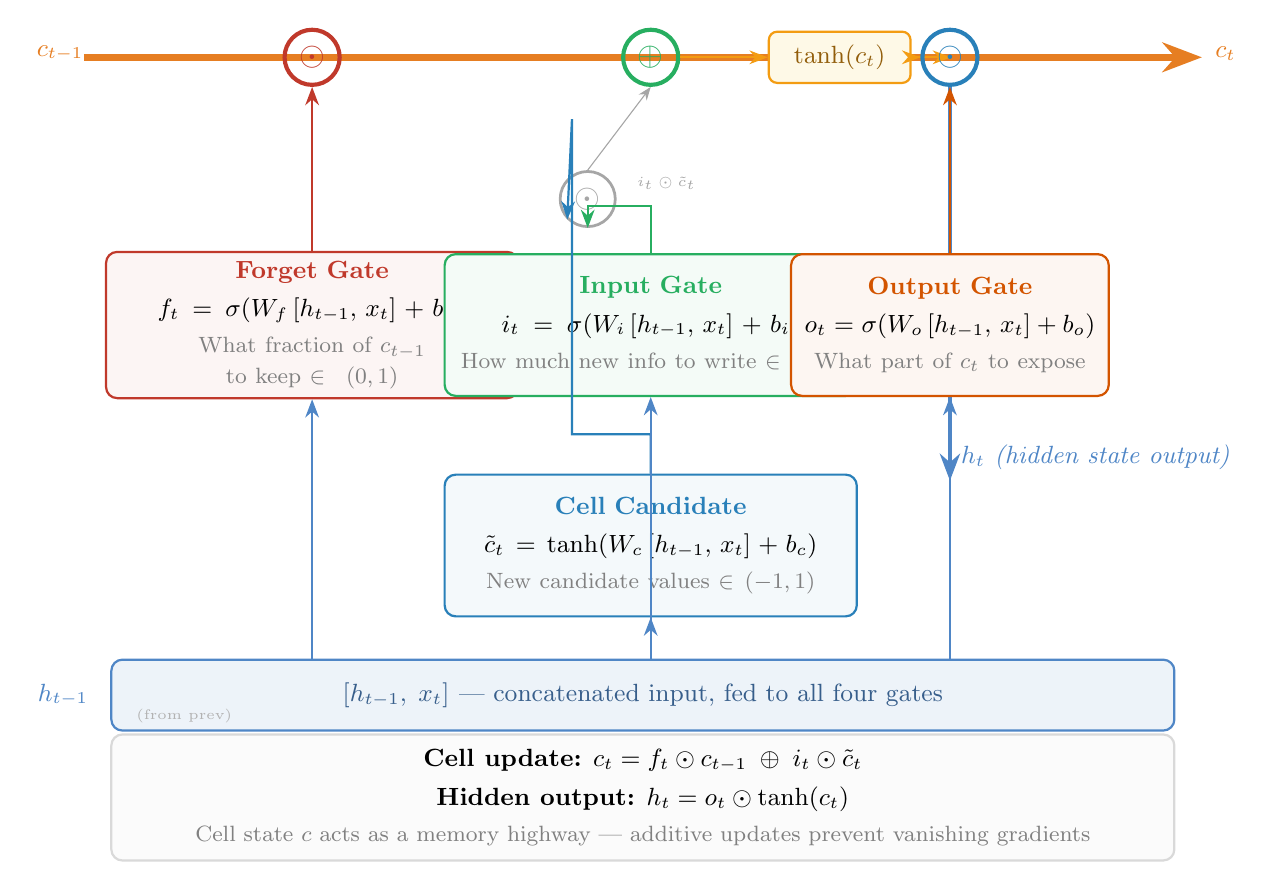
\begin{tikzpicture}[
  % arrow styles
  >=Stealth,
  thick,
  % gate box style
  gatebox/.style={
    draw, rounded corners=4pt, minimum width=5.2cm, minimum height=1.8cm,
    font=\small, align=center
  },
  % operator circle style
  opcirc/.style={
    draw, circle, minimum size=0.7cm, inner sep=0pt,
    font=\large, line width=1.5pt
  },
  % thin connector
  conn/.style={->, thin}
]

% ── Coordinate system: highway at y=0, everything below is negative y ───────

% ─── Cell-state highway ─────────────────────────────────────────────────────
\draw[highwayorange, line width=2.5pt, ->]
  (-0.4, 0) -- (13.8, 0);
\node[highwayorange, font=\itshape\small] at (-0.7, 0.05) {$c_{t-1}$};
\node[highwayorange, font=\itshape\small] at (14.1, 0.05) {$c_{t}$};

% ─── Operator nodes on the highway ─────────────────────────────────────────
% Forget-gate multiply  (red)
\node[opcirc, draw=forgetred, text=forgetred] (forget_mul) at (2.5, 0) {$\odot$};

% Add node  (green)
\node[opcirc, draw=inputgreen, text=inputgreen] (add_node) at (6.8, 0) {$\oplus$};

% tanh(c_t) box (amber)
\node[draw=tanhborder, fill=tanhbg, rounded corners=3pt,
      minimum width=1.8cm, minimum height=0.65cm,
      font=\small\bfseries, text=tanhborder!60!black] (tanh_ct)
  at (9.2, 0) {$\tanh(c_t)$};
\draw[tanhborder, ->] (add_node.east) -- (tanh_ct.west);
\draw[tanhborder, ->] (tanh_ct.east) -- ++(0.5,0);

% Output-gate multiply (blue)
\node[opcirc, draw=candidateblue, text=candidateblue] (out_mul)
  at (10.6, 0) {};
\node[font=\large, text=candidateblue] at (out_mul) {$\odot$};
% connect tanh to out_mul
\draw[tanhborder, ->] (tanh_ct.east) -- (out_mul.west);

% ─── h_t output: drop down from out_mul ─────────────────────────────────────
\draw[arrowblue, line width=1.5pt, ->]
  (out_mul.south) -- ++(0,-5.0)
  node[right, font=\itshape\small, text=arrowblue, yshift=0.3cm]
    {$h_t$ \small(hidden state output)};

% ─── Gate boxes ─────────────────────────────────────────────────────────────

% Forget Gate (red)
\node[gatebox, draw=forgetred, fill=forgetred!5,
      text width=5.0cm] (forget_box)
  at (2.5, -3.4) {
    \textcolor{forgetred}{\textbf{Forget Gate}}\\[3pt]
    $f_t = \sigma(W_f\,[h_{t-1},\,x_t] + b_f)$\\[2pt]
    \textcolor{gray}{\footnotesize What fraction of $c_{t-1}$ to keep $\in(0,1)$}
  };
\draw[forgetred, ->] (forget_box.north) -- (forget_mul.south);

% Input Gate (green)
\node[gatebox, draw=inputgreen, fill=inputgreen!5,
      text width=5.0cm] (input_box)
  at (6.8, -3.4) {
    \textcolor{inputgreen}{\textbf{Input Gate}}\\[3pt]
    $i_t = \sigma(W_i\,[h_{t-1},\,x_t] + b_i)$\\[2pt]
    \textcolor{gray}{\footnotesize How much new info to write $\in(0,1)$}
  };

% Cell Candidate (blue)
\node[gatebox, draw=candidateblue, fill=candidateblue!5,
      text width=5.0cm] (cand_box)
  at (6.8, -6.2) {
    \textcolor{candidateblue}{\textbf{Cell Candidate}}\\[3pt]
    $\tilde{c}_t = \tanh(W_c\,[h_{t-1},\,x_t] + b_c)$\\[2pt]
    \textcolor{gray}{\footnotesize New candidate values $\in(-1,1)$}
  };

% Output Gate (orange)
\node[gatebox, draw=outputorange, fill=outputorange!5,
      minimum width=4.0cm, text width=3.8cm] (output_box)
  at (10.6, -3.4) {
    \textcolor{outputorange}{\textbf{Output Gate}}\\[3pt]
    $o_t = \sigma(W_o\,[h_{t-1},\,x_t] + b_o)$\\[2pt]
    \textcolor{gray}{\footnotesize What part of $c_t$ to expose}
  };
\draw[outputorange, ->] (output_box.north) -- (out_mul.south);

% ─── Intermediate i_t ⊙ c̃_t node ────────────────────────────────────────────
\node[opcirc, draw=gray!70, text=gray!70, line width=1pt] (int_mul)
  at (6.0, -1.8) {$\odot$};
\node[font=\tiny, text=gray!70] at (7.0, -1.6) {$i_t \odot \tilde{c}_t$};

% input gate → intermediate ⊙
\draw[inputgreen, ->] (input_box.north) -- ++(0, 0.6) -| (int_mul.south);

% cell candidate → intermediate ⊙
\draw[candidateblue, ->]
  (cand_box.north) -- ++(0,0.5) -- ++(-1.0,0) -- ++(0,4.0)
  -- (int_mul.south west);

% intermediate ⊙ → ⊕ on highway
\draw[->, gray!70, thin] (int_mul.north) -- (add_node.south);

% ─── Input bar ──────────────────────────────────────────────────────────────
\node[draw=arrowblue, fill=arrowblue!10, rounded corners=4pt,
      minimum width=13.5cm, minimum height=0.9cm,
      font=\small\bfseries, text=arrowblue!70!black] (input_bar)
  at (6.7, -8.1) {
    $[h_{t-1},\; x_t]$ \normalfont--- concatenated input, fed to all four gates
  };

% label on left
\node[font=\itshape\small, text=arrowblue, left=0.15cm of input_bar]
  {$h_{t-1}$};
\node[font=\tiny, text=gray!60, below=0.05cm of input_bar.west, anchor=north west,
      xshift=0.2cm] {(from prev)};

% arrows from input bar to gates
\draw[arrowblue, ->] (2.5, -7.65) -- (forget_box.south);
\draw[arrowblue, ->] (6.8, -7.65) -- (input_box.south);
\draw[arrowblue, ->] (6.8, -7.65) -- (cand_box.south);
\draw[arrowblue, ->] (10.6,-7.65) -- (output_box.south);

% ─── Formula summary box ─────────────────────────────────────────────────────
\node[draw=gray!30, fill=gray!3, rounded corners=4pt,
      minimum width=13.5cm, minimum height=1.6cm,
      align=center, font=\small] (formula_box)
  at (6.7, -9.4) {
    \textbf{Cell update:} $c_t = f_t \odot c_{t-1} \;\oplus\; i_t \odot \tilde{c}_t$\\[3pt]
    \textbf{Hidden output:} $h_t = o_t \odot \tanh(c_t)$\\[2pt]
    \textcolor{gray}{\footnotesize Cell state $c$ acts as a memory highway --- additive updates prevent vanishing gradients}
  };

\end{tikzpicture}

\end{document}
